% This work is licensed under the Creative Commons
% Attribution-NonCommercial-ShareAlike 4.0 International License. To view a copy
% of this license, visit http://creativecommons.org/licenses/by-nc-sa/4.0/ or
% send a letter to Creative Commons, PO Box 1866, Mountain View, CA 94042, USA.
% vim: set noexpandtab:

\section{Finite-Elemente Räume} %4
\begin{definition}[1D finite Elemente]\enter
	Sei $\Omega=(0,1)\subseteq\R$. Sei
	\begin{align*}
		\mathcal{T}_n:=\big\lbrace I_j:0\leq j\leq n\big\rbrace\mit I_j:=\big(t_j,t_{j+1}\big)
	\end{align*}
	und
	\begin{align*}
		0=t_0<t_1<\ldots<t_n< t_{n+1}=1
	\end{align*}
	eine Zerlegung von $(0,1)$. Weiterhin setze
	\begin{align*}
		h_j:=t_{j+1}-t_j,\qquad h:=\max\limits_{0\leq j\leq n} h_j
	\end{align*}
	Für $k\in\N_0$ und $m\in\N_0$ definiere
	\begin{align*}
		S_h^{k,-1}&:=\Big\lbrace\varphi:[0,1]\to\R:\varphi\big|_{I_j}\in P_k,~0\leq j\leq n\Big\rbrace\\
		S_h^{k,m}&:=S_n^{k,-1}\cap C^m\big([0,1]\big)\\
		S_{h,0}^{k,m}&:=\Big\lbrace\varphi\in S_n^{k,m}:\varphi(0)=\varphi(1)=0\Big\rbrace
	\end{align*}
	Hierbei ist $P_k$ der Raum der Polynome von höchstens Grad $k$.\\
	Die Funktionen in $S_h^{k,m}$ heißen \textbf{finite-Elemente-Funktionen}.

	\begin{figure}[!ht]
		\begin{center}
			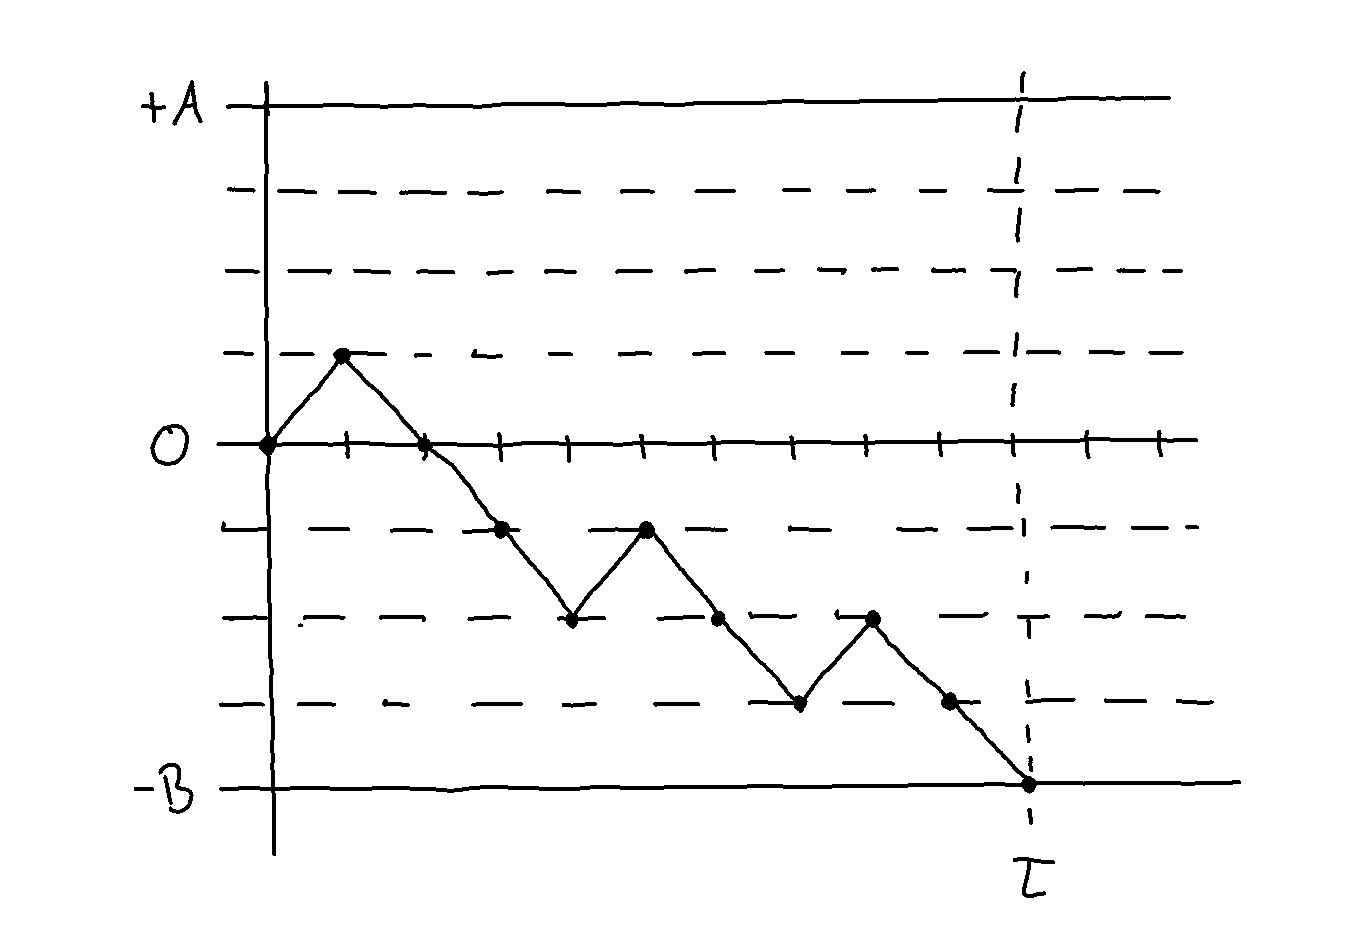
\includegraphics[width=0.75\textwidth]{pics/Sketch0.png}
			\caption{Beispiel für finite-Elemente-Funktionen}
			\label{AbbFiniteFunktionen}
		\end{center}
	\end{figure}
\end{definition}

\begin{bemerkung}\
	\begin{itemize}
		\item Für $m=k-1$ erhält man Splines.
		\item $\begin{aligned}
			S_h^{k,m}\subseteq H^{m+1}(\Omega)
		\end{aligned}$ wegen Satz \ref{satz1.4}
		\item $\begin{aligned}
			S_h^{0,m}
		\end{aligned}$ sind konstante Funktionen auf $(0,1)$ für $m\geq0$
		\item Die Räume haben folgende Dimensionen:
		\begin{align*}
			\dim\left(S_h^{k,-1}\right)&=(n+1)\cdot(k+1)\\
			\dim\left(S_h^{k,m}\right)&=\dim\left(S_h^{k,-1}\right)-n\cdot(m+1)\\
			\dim\left(S_{h,0}^{k,m}\right)&=\dim\left(S_h^{k,m}\right)-2\\
		\end{align*}
		Konkrete wichtige Beispiele:
		\begin{align*}
			\dim\left(S_h^{k,0}\right)&=(n+1)\cdot(k+1)-n\\
			\dim\left(S_{h,0}^{k,0}\right)&=(n+1)\cdot(k+1)-n-2=(n+1)\cdot(k-1)+n\\
			\dim\left(S_{h,0}^{1,0}\right)&=(n+1)\cdot 2-n-2=n\\
			\dim\left(S_{h,0}^{2,0}\right)&=(n+1)\cdot 3-n-2=2\cdot n+1\\
		\end{align*}
	\end{itemize}
\end{bemerkung}

Sei $\lbrace\varphi_j\rbrace_{j\in J}$ eine Basis von $S_h^{k,0}$
und Lösung $u_h\in S_{h,0}^{k,0}: u_h=\sum\limits_j u_j\cdot\varphi_j$\\
Diskretes Problem: Finde $u_h\in S_{h,0}^{k,0}$ so, dass
\begin{align*}
	&a(u_h,\varphi_h)=l(\varphi_h)&\qquad&\forall \varphi_h\in S_{h,0}^{k,0}\\
	\Longleftrightarrow &a(u_h,\varphi_i)=l(\varphi_i)&\qquad&\forall i
\end{align*}
In Matrix-Notation ergibt dies Folgendes:
\begin{align*}
	&A=(a_{i,j}),&&a_{i,j}:=a(\varphi_j,\varphi_i)\\
	&b=(b_i),&&b_i:=l(\varphi_i\nl
	&\qquad\Longleftrightarrow A\cdot U=b,\qquad U=(u_i)
\end{align*}
Hierbei heißt $A$ \textbf{Stiffness-Matrix}.

\begin{align*}
	S^{1,0}_{h,0}&=\text{span}\big\lbrace\varphi_i:1\leq i\leq n\big\rbrace,\qquad
	\varphi_i(t)=\left\lbrace\begin{array}{cl}
		\frac{t-t_{i-1}}{h_{i-1}}, &\falls t\in I_{i-1}\\
		\frac{t_{i+1}-t}{h_i}, &\falls t\in I_i\\
		0, &\sonst
	\end{array}\right.\\
	\big(\text{supp}(\varphi_i) &= [t_{i-1}, t_{i+1}]\big)\\
	\implies a_{i,j}&=0\text{ für }|i-j|>1\implies A\text{ ist Tridiagonalmatrix}
\end{align*}

\begin{figure}[!ht]
	\begin{center}
		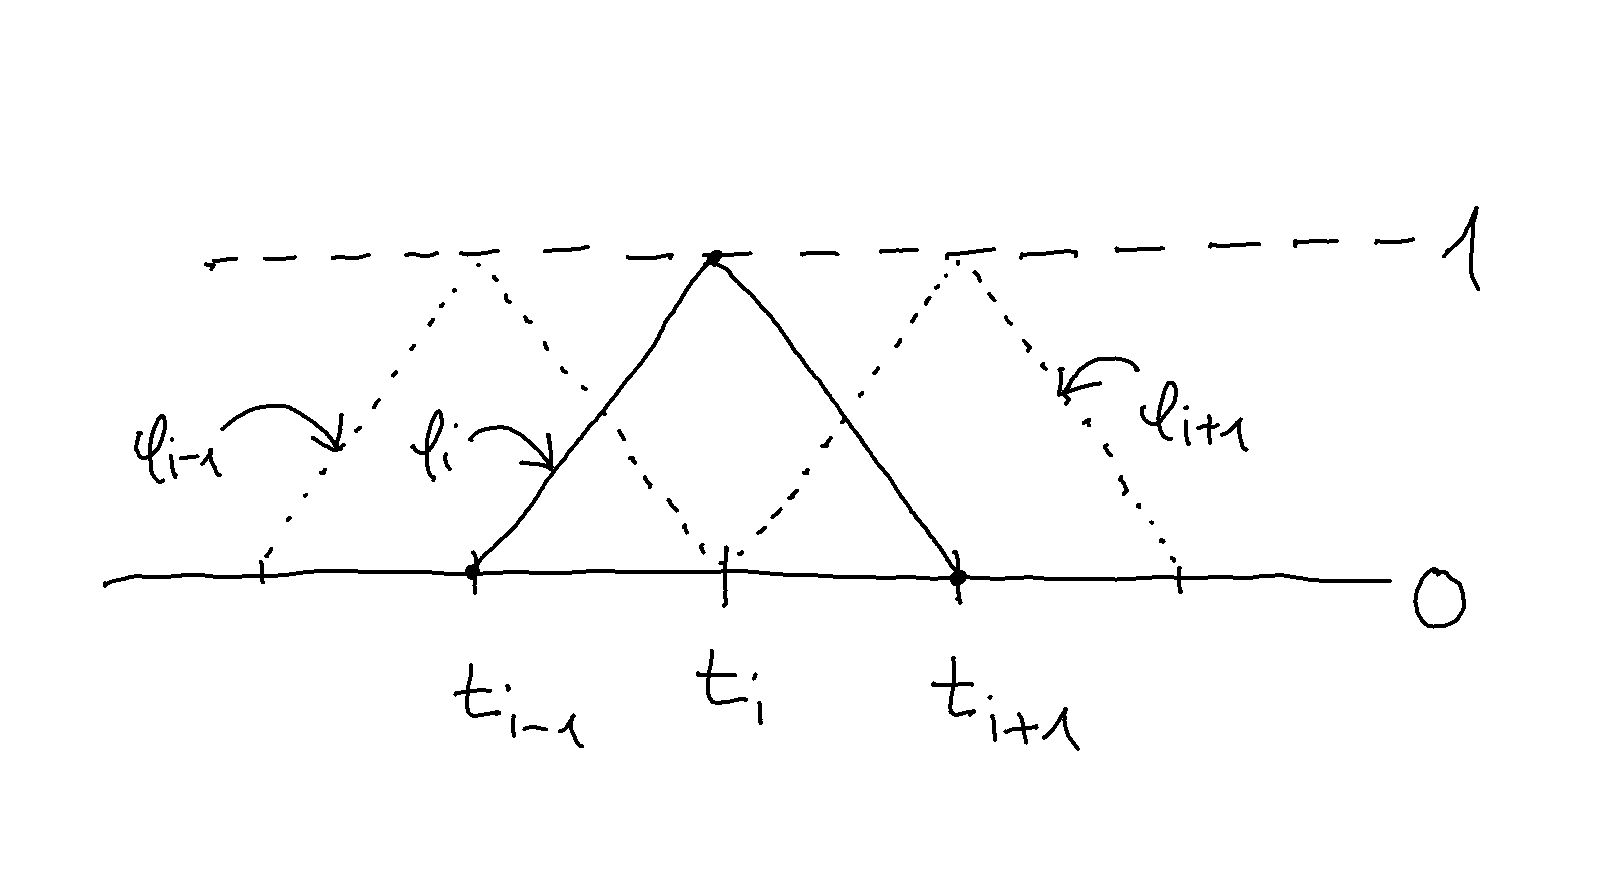
\includegraphics[width=0.75\textwidth]{pics/Sketch1.png}
		\caption{Hut-Funktionen}
		\label{AbbHutFunktionen}
	\end{center}
\end{figure}

\begin{figure}[!ht]
	\begin{center}
		\centering
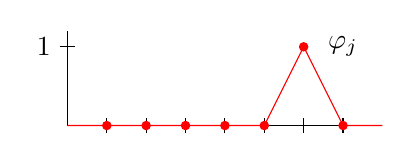
\begin{tikzpicture}[scale=1]

% Achsen
\draw (0,0) -- ++(0,1.2);
\draw (0,0) -- ++(4,0);

% Funktion
\draw[red] (0,0) -- ++(2.5,0) -- ++(0.5,1) -- ++(0.5,-1) -- ++(0.5,0);
	
% Anstrich Y-Achse 
\draw (-0.1,1) -- ++(0.2,0);
	
% Anstriche X-Achse
\draw (0.5,-0.1) -- ++(0,0.2);
\draw (1  ,-0.1) -- ++(0,0.2);
\draw (1.5,-0.1) -- ++(0,0.2);
\draw (2  ,-0.1) -- ++(0,0.2);
\draw (2.5,-0.1) -- ++(0,0.2);
\draw (3  ,-0.1) -- ++(0,0.2);
\draw (3.5,-0.1) -- ++(0,0.2);
	
	
\filldraw[red] (0.5,0) circle (1.5pt);
\filldraw[red] (1  ,0) circle (1.5pt);
\filldraw[red] (1.5,0) circle (1.5pt);
\filldraw[red] (2  ,0) circle (1.5pt);
\filldraw[red] (2.5,0) circle (1.5pt);
\filldraw[red] (3  ,1) circle (1.5pt);
\filldraw[red] (3.5,0) circle (1.5pt);
	
	
\node at (-0.3,1) {1};
\node at (3.5,1) {$\varphi_j$};
\end{tikzpicture}

		\caption{einzelne Hut-Funktion}
		\label{AbbPhiHat}
	\end{center}
\end{figure}

\begin{align*}
	S_{h,0}^{2,0}&=\spann\big\lbrace\varphi_1,\ldots,\varphi_n,\psi_0,\ldots,\psi_n\big\rbrace,\qquad
	\psi_i(t)=\left\lbrace\begin{array}{cl}
		4\cdot\frac{(t-t_i)\cdot(t_{i+1}-t)}{h_i^2}, &\falls t\in I_i\\
		0 &\sonst
	\end{array}\right.
\end{align*}

\begin{figure}[!ht]
	\begin{center}
		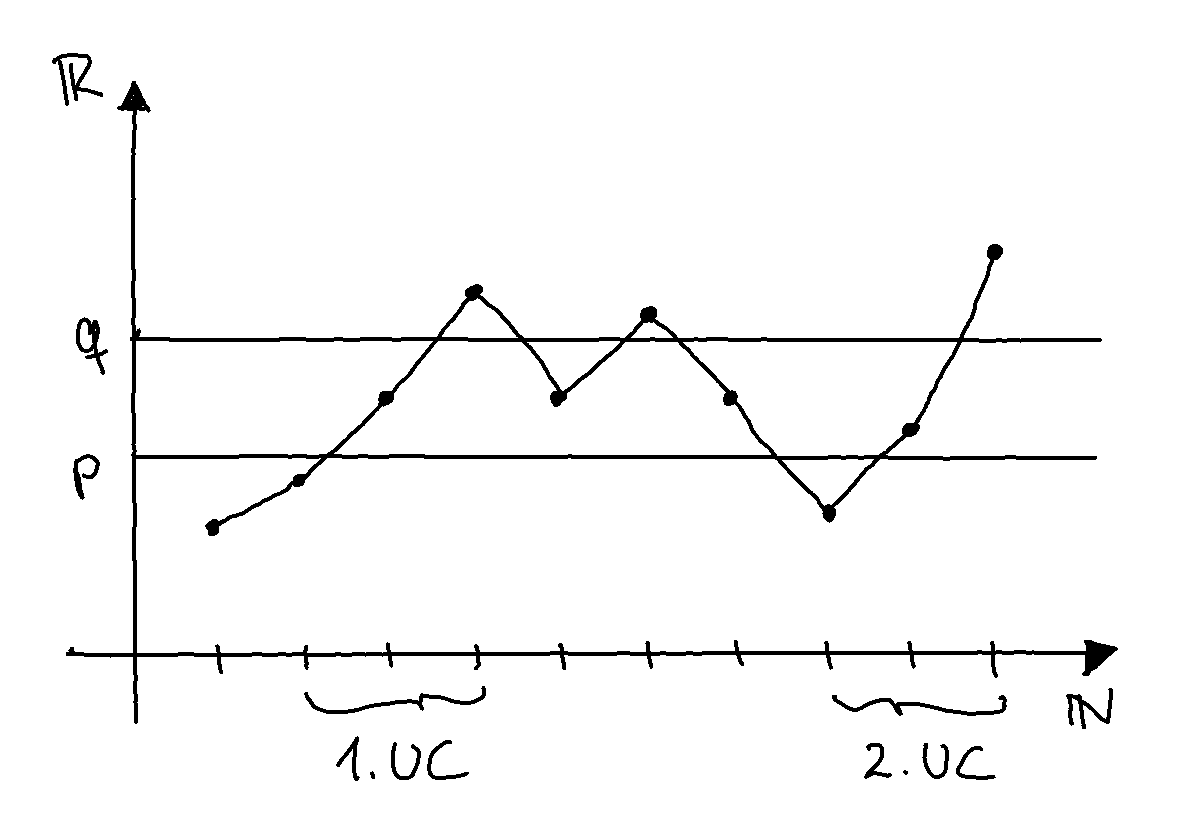
\includegraphics[width=0.5\textwidth]{./pics/Sketch2.png}
		\caption{einzelne zweifach diffbare finite-Elemente-Funktion}
		\label{AbbFiniteElementeFunktionZweifachDiffbar}
	\end{center}
\end{figure}

Die Stiffness-Matrix $A$ lässt sich als Blockmatrix schreiben:
\begin{align*}
	A=\begin{pmatrix}
		A_{LL} & A_{LQ}\\
		A_{QL} & A_{QQ}
	\end{pmatrix}
\end{align*}
wobei $A_{QQ}$ eine Diagonalmatrix ist. Somit:
\begin{align*}
	\begin{pmatrix}
		A_{LL} & A_{LQ}\\
		A_{QL} & A_{QQ}
	\end{pmatrix}\cdot\begin{pmatrix}
		U_L\\ U_Q
	\end{pmatrix}=
	\begin{pmatrix}
		b_L\\ b_Q
	\end{pmatrix}
\end{align*}
Dieses System von Gleichungen ist äquivalent zu:
\begin{align*}
	\big(A_{LL}-A_{LQ}\cdot A^{-1}_{QQ}\cdot A_{QL}\big)\cdot U_L&= b_L-A_{LQ}\cdot A^{-1}_{QQ}\cdot b_Q\\
	A_{QQ}\cdot U_Q&= b_Q-A_{QL}\cdot U_L
\end{align*}

\begin{theorem}[Approximationseigenschaft von 1D finiten Elementen]\label{theorem4.2}\enter
	Sei $u\in H^{k+1}(\Omega)\cap H^{1}_0(\Omega)$ für ein $k\geq1$. Dann gilt:
	\begin{align*}
		\inf\limits_{v_h\in S_{h,0}^{k,0}}\big|u-v_h\big|_{1,2}\leq h^k\cdot|u|_{k+1,2}
	\end{align*}
	(Hierbei ist $h$ wie oben der Maximalabstand.)
\end{theorem}

\begin{proof}
	Definiere Intervallweise die Funktion auf $I_i$ durch
	\begin{align*}
		v_h^\ast(t):=L_i(t)\qquad\forall t\in I_i,~\forall i\in\lbrace1,\ldots,n\rbrace
	\end{align*}
	wobei die $L_i$ die Lagrange-Interpolationen in $P_k$ bzgl. $t_i+\frac{s}{h}\cdot h_i,~0\leq j\leq h$ sind.\\
	Offenbar gilt $v_h^\ast\in S^{k,0}_{h,0}$. \\
	$u-v_n^\ast$ in $\overline{I_i}=[t_i,t_{i+1}]$ hat $(k+1)$ Nullen wegen der Interpolation. Somit hat $\big(u-v_h^\ast)^{(\mu)}$ $(k+1-\mu)$ Nullen.
	\begin{align*}
		\big|u-v_h^\ast\big|_{\mu,2,I_i}
		&=\left\Vert \big(u-v_h^\ast\big)^{(\mu)}\right\Vert_{0,2,I_i}\\
		&\stackrel{}{\leq}
		h_i\cdot\left|\big(u-v_h^\ast\big)^{(\mu)}\right|_{1,2,I_i}\\
		&=h_i\cdot\left|\big(u-v_h^\ast\big)^{(\mu+1)}\right|_{0,2,I_i}\\
		&\leq h_i\cdot\left|u-v_h^\ast\right|_{\mu+1,2,I_i}\\
		\implies
		\big|u-v_h^\ast\big|_{1,2,I_i}
		&\leq h_i^k\cdot\big|u-v_h^\ast\big|_{k+1,2,I_i} \\
		\overset{v_h^\ast|_{I_i}\in P_k}&=
		h_i^k\cdot |u|_{k+1,2,I_i}
	\end{align*}
	Somit folgt
	\begin{align*}
		\big| u-v_h^\ast\big|_{1,2,\Omega}
		&=\left(\sum\limits_{i=1}^n\big|u-v_h^\ast\big|^2_{1,2,I_i}\right)^{\frac{1}{2}}\\
		&\leq\left(\sum\limits_{i=1}^n \underbrace{h_i^{2\cdot k}}_{\leq h^{2\cdot k}} \big|u\big|^2_{k+1,2,I_i}\right)^{\frac{1}{2}}\\
		&\leq h^k\cdot |u|_{k+1,2,\Omega}
	\end{align*}
\end{proof}

\begin{lemma}\label{lemma4.3}
	Sei $u\in H^1((a,b))$ mit der Eigenschaft
	\begin{align*}
		\exists t^\ast\in[a,b]:u(t^\ast)=0.
	\end{align*}
	Dann gilt:
	\begin{align*}
		\Vert  u\Vert_{L^\infty}:=\max\limits_{t\in [a,b]}\big|u(t)\big|&\leq(b-a)^{\frac{1}{2}}\cdot |u|_{1,2}\\
		\Vert u\Vert_{0,2}&\leq(b-a)\cdot|u|_{1,2}
	\end{align*}
	Für alle $u\in H^1_0((a,b))$ gilt:
	\begin{align*}
		\left(1+(b-a)^2\right)^{\frac{1}{2}}\cdot\Vert u\Vert_{1,2}\leq|u|_{1,2}\leq\Vert u\Vert_{1,2}
	\end{align*}
\end{lemma}

\subsection*{Sturm-Liouville Problem}
\begin{align}\label{eqSturmLiouvillePDE}\tag{SturmLiouville}
	\left\lbrace\begin{array}{rll}
		-\big(p(x)\cdot u'(x)\big)'+q(x)\cdot u(x) &= f(x) &\text{ in } (0,1)\\
		u(0)=u(1)&=0 &
	\end{array}
	\right.
\end{align}
wobei
\begin{align*}
	&f\in L^2((0,1)),\\
	&q\in C\big([0,1]\big), &&q(x)\geq0\quad\forall x\in[0,1], \\
	&p\in C\big([0,1]\big), &&p(x)\geq p_0>0\quad\forall x\in [0,1]
\end{align*}
\begin{align*}
	a(v,w)=\int\limits_0^1 p(x)\cdot v'(x)\cdot w'(x)+q(x)\cdot v(x)\cdot w(x)\d x
\end{align*}

\begin{theorem}\label{theorem4.4}
	Sei $u\in H^1_0\big((0,1)\big)$ die eindeutige schwache Lösung von \eqref{eqSturmLiouvillePDE} und $u_h$ die zugehörige Lösung in $S_{h,0}^{k,0}$.
	Falls $u\in H^{k+1}\big((0,1)\big)$, dann gilt:
	\begin{align*}
		|u-u_h|_{1,2}&\leq c_1\cdot h^k\cdot |u|_{k+1,2}\\
		\Vert u-u_h\Vert_{0,2}&\leq c_1\cdot h^k\cdot |u|_{k+1,2}\\
		\mit c_1&=\frac{2}{p_0}\cdot\max\limits\big\lbrace \Vert p\Vert_{C^0},\Vert q\Vert_{C^0}\big\rbrace
	\end{align*}
	Falls zusätzlich die schwache Formulierung für alle $\varphi\in L^2\big((0,1)\big)$ eine eindeutige schwache Lösung
	\begin{align*}
		u_\varphi\in H^2\big((0,1)\big)\cap H^1_0\big((0,1)\big)\mit |u_\varphi|_{2,2}\leq c_2\cdot\Vert \varphi\Vert_{0,2}
	\end{align*}
	liefert, dann gilt
	\begin{align*}
		\big\Vert u-u_h\big\Vert_{0,2}\leq c_3\cdot h^{k+1}\cdot |u|_{k+1,2}
		\mit c_3=\frac{4\cdot c_2}{p_0}\cdot\max\limits\left\lbrace\Vert p\Vert^2_{C^0},\Vert q\Vert^2_{C^0}\right\rbrace
	\end{align*}
\end{theorem}

Nun der zweidimensionale Fall: Sei $\Omega\subseteq\R^2$ ein beschränktes Polygon. Nun zerlegen wir das Polygon in Dreiecke. Dieses Verfahren heißt \textbf{Dekomposition / Triangulierung.} Dadurch erhalten wir eine Menge von \underline{offenen} (nach Konvention) Dreiecken $\lbrace K_i\rbrace_{i\in\lbrace1,\ldots,N\rbrace}$ mit den Eigenschaften:

\begin{enumerate}[label=(\roman*)]
	\item $\begin{aligned}
		\overline{\Omega}=\bigcup\limits_{i=1}^N \overline{K_i}
		\end{aligned}$
	\item $\begin{aligned}
		i\neq j\implies K_i\cap K_j=\emptyset
	\end{aligned}$
	\item Zulässigkeit: $\overline{K_i}\cap\overline{K_j}$ für $i\neq j$ ist
	\begin{itemize}
		\item leer oder
		\item ein einziger Punkt oder
		\item eine \ul{gemeinsame} Kante.
	\end{itemize}

	\begin{figure}[!ht]
		\begin{center}
			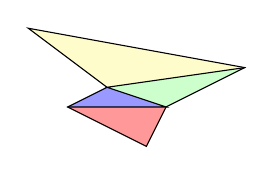
\begin{tikzpicture}[scale=1]

     
	
    % fill triangles
    \fill[red!40!white]   (0,0) -- ++(1,-0.5) -- ++(0.25,0.5) --cycle;
    \fill[blue!40!white]  (0,0) -- ++(1.25,0) --++(-0.75,0.25) --cycle;
    \fill[green!20!white]   (1.25,0) --++(-0.75,0.25) --++(1.75,0.25) --cycle;
    \fill[yellow!20!white]   (0.5,0.25) --++(1.75,0.25) --  ++(-2.75,0.5) --cycle;
	 
	% outline
	\draw (0,0) -- ++(1,-0.5) -- ++(0.25,0.5)-- ++(1,0.5) -- ++(-2.75,0.5)-- ++(1,-0.75)--cycle;

	% this is unrobust
	\draw (0,0) -- ++(1.25,0) --++(-0.75,0.25) --++(1.75,0.25);

\end{tikzpicture}
			\caption{beispielhafte Triangluierung, $K_i$ disjunkt}
			\label{AbbTriangulierung}
		\end{center}
	\end{figure}

	\begin{figure}[!ht]
		\begin{center}
			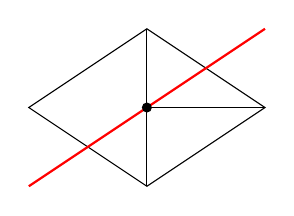
\begin{tikzpicture}[scale=1]

	% outline
	\draw (0,0) -- ++(1.5,-1) -- ++(1.5,1)-- ++(-1.5,1) -- cycle;
	\draw (1.5,-1) -- ++(0,2);
	\draw (1.5,0) -- ++(1.5,0);
	
	% red cross
	\draw[thick,red] (0,-1) --++ (3,2);

	% dot middle
	\filldraw (1.5,0) circle (1.6pt);

\end{tikzpicture}
			\caption{Unzulässige Triangulierung}
			\label{AbbUnzulaessigeTriangulierung}
		\end{center}
	\end{figure}
\end{enumerate}

\subsection*{Raum der stetigen stückweise linearen Funktionen}
\begin{align*}
	V_h&:=\left\lbrace
	\begin{array}{rl}
		v\in C(\overline{\Omega}) : &v|_{K_i}\in P_1(K)~\forall i=1,\ldots,N,\\
		&v|_{\partial\Omega}=0
	\end{array}\right\rbrace
	\subseteq H^1_0(\Omega)\\
	P_1(K_i)&=\spann(1,x,y)\\
	P_2(K)&=\spann\big( x^\alpha, |\alpha|\leq k\big)\mit K\subseteq\R^d,~ x^{\alpha}:=x_1^{\alpha_1},\ldots,x_d^{\alpha_d}\\
	Q_k(K)&=\spann\big(x^\alpha,\max\limits_i |\alpha_i|\leq k\big)\\
	Q_1(K)&=\spann(1,x,y,xy)\\
	\dim(V_h)&=\text{ Anzahl der inneren Knoten von der zulässigen Triangulierung}\\
\end{align*}

\begin{definition}[Finites Element]\enter %4.5
	Ein \textbf{finites Element} ist ein Tripel $(K,V,\Sigma)$ mit:
	\begin{enumerate}[label=(\roman*)]
		\item $K\subseteq\R^d$ ist nichtleere offene, beschränkt und Lipschitz-berandet.
		\item $V$ ist endlich-dimensionaler Funktionenraum von Funktionen mit Definitionsbereich $K$. $m:=\dim(V)$
		\item $\Sigma$ ist eine Menge von $m$ linearen Funktionalen $\Sigma=\lbrace N_i\rbrace_{i\in\lbrace1,\ldots,m\rbrace}$, welche mindestens für alle 	 Funktionen in $V$ definiert sind.
		Sie werden als \textbf{$V$-unisolvent} angenommen, d. h.:
		\begin{align*}
			\forall \alpha_1,\ldots\alpha_m:\exists! v\in V:\forall i\in\lbrace1,\ldots,m\rbrace:N_i(v)=\alpha_i
		\end{align*}
		Das bedeutet, es gibt Funktionen $v_i\in V$ mit
		\begin{align*}
			N_i(v_j)=\delta_{i,j}\qquad\forall i,j\in\lbrace1,\ldots m,\rbrace
		\end{align*}
		Die linearen Funktionale $N_i$ heißen \textbf{Nodal-Funktionen} oder \textbf{Freiheitsgrade (degrees of freedom / dof)}.
		Die Funktionen $v_i$ sind die \textbf{lokale Basis} oder \textbf{Shape-Funktionen / Formfunktionen}.
	\end{enumerate}
\end{definition}

\begin{definition}[affin äquivalente finite Elemente]\enter %4.6
	Zwei finite Elemente $(K,V,\Sigma)$ und $(\hat{K},\hat{V},\hat{\Sigma})$ heißen \textbf{affin äquivalent}
	\begin{align*}
		:\Longleftrightarrow\exists F:\R^d\to\R^d\text{ affin \& invertierbar v.d.F. }
		\hat{x}\mapsto B_k\cdot\hat{x}+b_k\mit B_k\in\R^{d\times d},b_k\in\R^d
	\end{align*}
	mit den Eigenschaften
	\begin{enumerate}[label=(\arabic*)]
		\item $\begin{aligned}
			K=F(\hat{K})
		\end{aligned}$
		\item $\begin{aligned}
			V=\Big\lbrace v: K\to\R:v=\hat{v}\circ F^{-1},\hat{v}\in\hat{V}\Big\rbrace
		\end{aligned}$
		\item $\begin{aligned}
			\Sigma=\Big\lbrace N:V\to\R:N(v)=\hat{N}(v\circ F),~\hat{N}\in\hat{\Sigma}\Big\rbrace
		\end{aligned}$
	\end{enumerate}
\end{definition}

\begin{beisp}\
	\begin{figure}[!ht]
		\begin{center}
			\centering
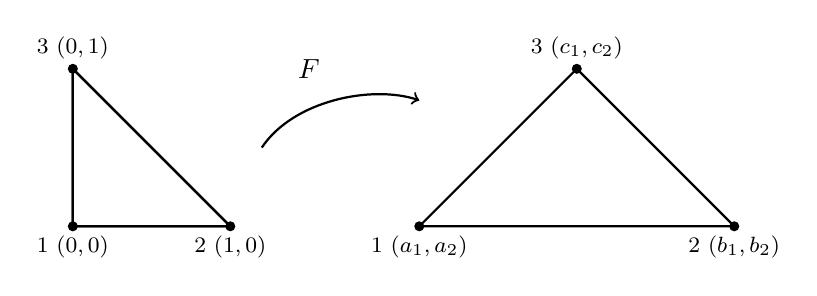
\begin{tikzpicture}[scale=2]


\draw[thick] (0,0) -- ++(0,1) -- ++(1,-1)--cycle;
\filldraw (0,0)         circle (0.8pt);
\filldraw (0,0) ++(1,0) circle (0.8pt);
\filldraw (0,0) ++(0,1) circle (0.8pt);
\fill[black,font=\footnotesize] (0,0) node[below] {1 $(0,0)$}
								(0,0) ++(1,0) node[below] {2 $(1,0)$}
								(0,0) ++(0,1) node[above] {3 $(0,1)$};
								
\draw[thick] (2.2,0) -- ++(2,0) -- ++(-1,1)--cycle;
\filldraw (2.2,0)         circle (0.8pt);
\filldraw (2.2,0) ++(2,0) circle (0.8pt);
\filldraw (2.2,0) ++(1,1) circle (0.8pt);
\fill[black,font=\footnotesize] (2.2,0) node[below] {1 $(a_1,a_2)$}
								(2.2,0) ++(2,0) node[below] {2 $(b_1,b_2)$}
								(2.2,0) ++(1,1) node[above] {3 $(c_1,c_2)$};								
								
												
\node at (1.5,1) {$F$};				
\draw[thick,-to] (1.2,0.5) .. controls (1.4,0.8) and (1.9,0.9) .. (2.2, 0.8);
\draw[thick] (0,0) -- ++(0,1) -- ++(1,-1)--cycle;

\end{tikzpicture}

			\caption{affin äquivalente Triangulierung}
			\label{AbbAffinEquivTriang}
		\end{center}
	\end{figure}

	\begin{align*}
		F:\left\lbrace\begin{array}{l}
			(0,0)\mapsto(a_1,a_2)\\
			(1,0)\mapsto(b_1,b_2)\\
			(0,1)\mapsto(c_1,c_2)
		\end{array}\right.
		\qquad\qquad
		\begin{matrix}
			\hat{N}_1(\hat{v})&=\hat{v}(0,0) &&N_1(v)=v(a_1,a_2)\\
			\hat{N}_2(\hat{v})&=\hat{v}(1,0) &&N_2(v)=v(b_1,b_2)\\
			\hat{N}_3(\hat{v})&=\hat{v}(0,1) &&N_3(v)=v(c_1,c_2)
		\end{matrix}
	\end{align*}
\end{beisp}

Sei $V$ ein Vektorraum mit Basis $\lbrace\varphi_1,\ldots,\varphi_m\rbrace$. Setze
\begin{align*}
	\Sigma&=\lbrace N_1,\ldots,N_m\rbrace\\
	M&=(m_{i,j}),\qquad m_{i,j}:=N_i(\varphi_j)\\
	M&\text{ invertierbar }\Longleftrightarrow \text{ unisolvent}
\end{align*}
Unisolvenz: Gegeben $\alpha_1,\ldots\alpha_m\in\R$. Gibt es ein eindeutiges $v\in V$
\begin{align*}
	N_i(v)&=\alpha_i,\qquad i\in\lbrace1,\ldots,m\rbrace\\
	\stackrel{v=\sum\limits_{j=1}^m c_j\cdot\varphi_j}{\Longleftrightarrow}\quad
	\sum\limits_{j=1}^m N_i(\varphi_j)\cdot c_j&=\alpha_i\\
	\Longleftrightarrow
	M\cdot c&=\alpha
\end{align*}

\begin{definition}[globales Nodal-Funktional / globale Freiheitsgrade (dof)]\enter
	Seien $N_i^K$ und $N_j^{K'}$ zwei lokale Nodal-Funktionale von den finiten Elementen $(K,V,\Sigma)$ und $(K',V',\Sigma')$.
	Wir sagen, diese beiden lokalen Freiheitsgrade \textbf{gehören zum selben globalen Freiheitsgrad}
	\begin{align*}
		:\Longleftrightarrow N_i^K(\varphi|_K)=N_j^{K'}(\varphi|_{K'})\qquad\forall\varphi\in C^\infty(U)
	\end{align*}
	wobei $U$ eine offene Menge mit der Eigenschaft $\overline{K\cup K'}\subseteq U$ ist.\\
	Die Menge aller globalen Freiheitsgrade bezeichnen wir mit $\Sigma_h$.
	Für $N\in\Sigma_h$ bezeichne $\Lambda(N)$ die Menge alle lokalen Freiheitsgrade, die zu $N$ gehören.
\end{definition}

\begin{definition}[Raum der finiten Elemente]\enter
	Sei $\T_h$ eine Triangulierung von $\Omega$. Ein \textbf{Raum der finiten Elemente} $V_h$ ist gegeben durch
	\begin{align*}
		V_h:=\left\lbrace v=(v_{K})_{K\in\T_h}\in\prod\limits_{K\in\mathcal{T}_h} V(K):
		\begin{array}{cl}
			N_i^K(v|_K)=N_j^{K'}(v|_{K'}) &\forall N_i^K\\
			N_j^{K'}\in\Lambda(N) &\forall N\in\Sigma_h
		\end{array}
		\right\rbrace
	\end{align*}
	wobei $(K,V(K),\Sigma(K)),K\in\T_h$ finite Elemente sind.
	Eine Funktion $v_h\in V_h$ ist eindeutig bestimmt durch die Werte von $N(v_h)$ von dem globalen Freiheitsgrad.
\end{definition}

Familie aller affin äquivlenten finiten Elementen
\begin{align*}
	\big(K,V(K),\Sigma(K)\big)\sim\big(\hat{K},\hat{V},\hat{\Sigma}\big)
\end{align*}
Interpolation:
\begin{align*}
	I_h(v):=\sum\limits_{i=1}^n N_i(v)\cdot\varphi_i\in V_h
\end{align*}
wobei $\Sigma_h=\lbrace N_1,\ldots,N_n\rbrace\text{ und }\lbrace\varphi_1,\ldots,\varphi_n\rbrace$ eine Basis von $V_h$ ist mit der Eigenschaft $N_i(\varphi_j)=\delta_{i,j}$.\nl
\textbf{Wichtig: }
\begin{align*}
	\big(I_h(v)\big)\big|_K&=I_h^K\big(v|_K\big)\quad\text{wobei}\\ I_h^K(v)&=\sum\limits_{i=1}^{m_K} N_i^{(K)}(v)\cdot\varphi_i^K,\qquad N_i^K(\varphi_j^K)=\delta_{i,j}\qquad\Sigma(K)=\left\lbrace N_1^K,\ldots,N_{m_K}^K\right\rbrace
\end{align*}

\begin{theorem}\label{theorem4.9}
	Seien $K,\hat{K}\subseteq\R^d$ zwei affin äquivalente offene  Teilmengen des $\R^d$, d. h. es existiert eine affine bijektive Abbildung
	\begin{align*}
		F:\hat{K}\to K,\qquad \hat{x}\mapsto B_K\cdot\hat{x}+ b_K\qquad\mit B_K\in\R^{d\times d}\text{ invertierbar und }b_K\in\R^d
	\end{align*}
	Falls $v\in W^{m,p}(K)$ für $m\geq0,p\in[1,\infty)$, dann gehört $\hat{v}:=v\circ F$ zu $W^{m,p}(\hat{K})$ und wir erhalten
	\begin{align*}
		\big|\hat{v}\big|_{m,p,\hat{K}}\leq c\cdot\Vert B_K\Vert^m\cdot\big|\det(B_K)\big|^{-\frac{1}{p}}\cdot|v|_{m,p,K}
	\end{align*}
	wobei $c=c(m,d)$ eine Konstante ist und $\Vert\cdot\Vert$ eine Matrixnorm, die durch die euklidische Vektornorm induziert wird.\\
	Zusätzlich gilt:
	\begin{align*}
		|v|_{m,p,K}&\leq c\cdot\Vert B_K^{-1}\Vert^m\cdot\big|\det(B_K)\big|^{\frac{1}{p}}\cdot|\hat{v}|_{m,p,\hat{K}}\\
		F^{-1}(x)&=B_K^{-1}\cdot x-B_K^{-1}\cdot b_K
	\end{align*}
\end{theorem}

\begin{lemma}\label{lemma4.10}
	Seien $K,\hat{K}$ affin äquivalent mit $F(\hat{x})=B_K\cdot\hat{x}+b_K$. Dann gilt:
	\begin{align*}
		\Vert B_K\Vert&\leq\frac{h_K}{\hat{\rho}},\qquad\Vert B_K^{-1}\Vert\leq\frac{\hat{h}}{\rho_K}\qquad\text{wobei}\\
		h_K&:=\diam(K):=\sup\limits_{x,y\in K}\Vert x-y\Vert\\
		\rho_K&:=\sup\big\lbrace\diam(S):S\subseteq K\text{ Sphäre}\big\rbrace
	\end{align*}
\end{lemma}

\begin{proof}
	\begin{align*}
		\Vert B_K\Vert&=\sup\limits_{z\neq0}\frac{\Vert B_K \cdot z\Vert}{\Vert z\Vert}=\frac{1}{\hat{\rho}}\cdot\sup\limits_{\Vert z\Vert=\hat{\rho}}\Vert B_K \cdot z\Vert
	\end{align*}
	Für alle $\eta$ mit $\Vert \eta\Vert=\hat{\rho}$ existieren zwei Punkte $\hat{x},\hat{y}\in\hat{K}$ so, dass $\eta=\hat{x}-\hat{y}$. Seien $x=F(\hat{x}),y=F(\hat{y})$. Dann gilt:
	\begin{align*}
		x-y&=B_K\cdot\hat{x}+b_K-\big(B_K\cdot\hat{y}+b_K\big)=B_K\cdot(\hat{x}-\hat{y})=B_K \cdot \eta\\
		\Vert B_K\cdot \eta\Vert&=\Vert x-y\Vert\leq h_K\\
		\implies \Vert h_K\Vert&\leq\frac{1}{\hat{\rho}}\cdot\sup\limits_{\Vert y\Vert=\hat{\rho}}\underbrace{\Vert B_K\cdot \eta\Vert}_{\leq h_K}\leq\frac{h_K}{\hat{\rho}}
	\end{align*}
\end{proof}

\begin{lemma}[Deny-Lions]\label{lemma4.11DenyLions}\enter
	Sei $P_r(K)$ der Raum aller Polynome mit höchstens Grad $r$. Dann gilt:
	\begin{align*}
		\exists c(K)>0:\inf\limits_{p\in P_r(K)}\Vert v+p\Vert_{r+1,p,K}\leq c(K)\cdot |v|_{r+1,p,K}\qquad\forall v\in W^{r+1,p}(K)
	\end{align*}
\end{lemma}

\begin{proof}
	\begin{align*}
		n:=\dim \big(P_r(K)\big)=\begin{pmatrix}
			r+d\\ d
		\end{pmatrix}\text{ (Binomialkoeffizient)}
	\end{align*}
	Setze  für $\alpha\in\N_0^d\mit|\alpha|\leq r $:
	\begin{align*}
		N_\alpha:W^{r+1,p}(K)\to\R,\qquad v\mapsto\int\limits_K D^\alpha v\d x\\
		\alpha\longleftrightarrow x^\alpha =\prod\limits_{i=1}^d x_i^{\alpha_i}
	\end{align*}
	Also ist $\big\lbrace N_\alpha:|\alpha|\leq r\big\rbrace$ unisolvent auf $P_r(K)$.
	\begin{align*}
		\implies\left.
		\begin{array}{cl}
			N_\alpha(p)=0, &\forall |\alpha|\leq r \\
			p\in P_r(K)&
		\end{array}
		\right\rbrace
		\implies p\equiv 0
	\end{align*}
	Wir werden die Ungleichung
	\begin{align}\label{eqProof4.11Stern}\tag{$\ast$}
		\Vert v\Vert_{r+1,p,K}\leq c(K)\cdot\left(|v|_{r+1,p,K}+\sum\limits_{|\alpha|\leq r}\big|N_\alpha (r)\big|\right)\qquad\forall v\in W^{r+1,p}(K)
	\end{align}
	indirekt zeigen. Angenommen, diese Ungleichung gilt nicht. Dann gibt es eine Folge $(v_l)_{l\in\N}$ mit
	\begin{align}
		\Vert v_l\Vert_{r+1,p,K}=1\qquad\forall l\in\N\nonumber\\
		\lim\limits_{l\to\infty} \left(|v|_{r+1,p,K}+\sum\limits_{|\alpha|\leq r}\big|N_\alpha (r)\big|\right)=0\label{eqProof4.11SternStern}\tag{$\ast\ast$}
	\end{align}
	Mit der kompakten Einbettung $W^{r+1,p}(K)\stackrel{c}{\hookrightarrow} W^{r,p}(K)$ erhalten wir:\\
	Es gibt eine Teilfolge $(v_m)_{m\in\N}\subseteq(v_l)_{l\in\N}$, die in $W^{r,p}(K)$ gegen $v\in W^{r,p}(K)$ konvergiert.\\
	Aus \eqref{eqProof4.11SternStern} folgt
	\begin{align*}
		\lim\limits_{m\to\infty}|v_m|_{r+1,p,K}=0\\
	\end{align*}
	Folglich ist $(v_m)_{m\in\N}$ eine Cauchyfolge in $W^{r+1,p}(K)$.
	Da $W^{r+1,p}(K)$ ein Banachraum und damit vollständig ist, konvergiert diese Folge: $v_m\stackrel{m\to\infty}{\longrightarrow} v\in W^{r+1,p}(K)$ und somit $|v|_{r+1,p,K}=0$.
	Also $v\in P_r(K)$.
	\begin{align*}
		\stackrel{\eqref{eqProof4.11SternStern}}{\implies}
		\left.\begin{array}{ll}
			&N_\alpha(v)=0\qquad\forall |\alpha|\leq r\\
			& v\in P_r(K)
		\end{array}\right\rbrace\implies v \equiv 0
	\end{align*}
	Dies ist ein Widerspruch zu $\Vert v\Vert_{r+1,p,K}=1$. Also folgt \eqref{eqProof4.11Stern}.\\
	Für jedes $v\in W^{r+1,p}(K)$ gibt es ein $q\in P_r(K)$ so, dass
	\begin{align*}
		N_\alpha(v)=-N_\alpha(q)\qquad\forall|\alpha|\leq r
	\end{align*}
	Es folgt
	\begin{align*}
		\inf\limits_{p\in P_r(K)}\Vert v+p\Vert_{r+1,p,K}
		&\leq\Vert v+q\Vert_{r+1,p,K}\\
		&\overset{\eqref{eqProof4.11Stern}}{\leq}
		c(K)\cdot\Big(\underbrace{|v+p|_{r+1,p,K}}_{=|v|_{r+1,p,K}}+\sum\limits_{|\alpha|\leq r}\underbrace{|N_\alpha(\cdot v+q)|}_{=0}\Big)
	\end{align*}
\end{proof}

\begin{lemma}[Bramble-Hilbert]\label{lemma4.12BrambleHilbert}
	Sei $(Y,\Vert\cdot\Vert_Y)$ ein Banachraum und $F:W^{r+1,p}(K)\to Y$ linear mit den Eigenschaften
	\begin{enumerate}[label=(\roman*)]
		\item $\begin{aligned}
			\big\Vert F(u)\Vert_Y\leq c_1\cdot\Vert u\Vert_{r+1,p,K}\qquad\forall u\in W^{r+1,p}(K)
		\end{aligned}$ mit $c_1$ unabhängig von $u$.
		\item $\begin{aligned}
			F(p)=0\qquad\forall p\in P_r(K)
		\end{aligned}$
	\end{enumerate}
	Dann gibt es Konstanten $c,\tilde{c}>0$ so, dass
	\begin{align*}
		\big\Vert F(u)\big\Vert_Y
		\leq c\cdot\inf\limits_{p\in P_r(K)}\Vert u+p\Vert_{r+1,p,K}
		\leq
		\tilde{c}\cdot |u|_{r+1,p,K}\qquad\forall u\in W^{r+1,p}(K)
	\end{align*}
\end{lemma}

\begin{proof}
	\begin{align*}
		F(u)
		\overset{\text{Lin+(ii)}}&=
		F(u+p)\qquad\forall p\in P_r(K)\\
		\big\Vert F(u)\big\Vert
		&=\inf\limits_{p\in P_r(K)}\Vert F(u+p)\big\Vert_Y\\
		\overset{\text{(i)}}&{\leq}
		c_1\cdot\inf\limits_{p\in P_r(K)}\Vert u+p\Vert_{r+1,p,K}\\
		\overset{\ref{lemma4.11DenyLions}}&{\leq}
		\tilde{c}\cdot |u|_{r+1,p,K}
	\end{align*}
\end{proof}

\begin{lemma}\label{lemma4.13}
	Seien $(\hat{K},\hat{V},\hat{\Sigma})$ und $(K,V,\Sigma)$ zwei affin-äquivalente Finite-Elemente wobei
	\begin{align*}
		F_k:\hat{K}\to K,\qquad\hat{x}\mapsto B_K\hat{x}+b_K
	\end{align*}
	Dann gilt:
	\begin{align*}
		(I_K v)\circ F_k=\hat{I}(v\circ F_K)
	\end{align*}
	wobei $\hat{I}$ und $I_K$ die Interpolations-Operatoren auf $\hat{K}$ bzw. $K$.
\end{lemma}

\begin{proof}
	(Nur Beweisidee, da zu technisch.)
	Nutze:
	\begin{align*}
		\hat{I}\hat{v}&=\sum\limits_{i=1}^m\hat{N}_i(\hat{v})\cdot\hat{\varphi}_i\\
		I_K v&=\sum\limits_{i=1}^m N_i(v)\cdot\varphi\\
		\varphi_i\circ F_K&=\hat{\varphi}\\
		N(v)&=\hat{N}(v\circ F_K)
	\end{align*}
\end{proof}

\begin{theorem}\label{theorem4.14}
	Seien $(\hat{K},\hat{V},\hat{\Sigma})$ Finites-Element, $m,r\in\N_0$ und $p,q\in[1,\infty]$ so, dass
	\begin{enumerate}[label=(\roman*)]
		\item $\begin{aligned}
			W^{r+1,p}(\hat{K})\hookrightarrow W^{m,q}(\hat{K})
		\end{aligned}$
		\item $\begin{aligned}
			P_r(\hat{K})\subseteq\hat{V}\subseteq W^{m,q}(\hat{K})
		\end{aligned}$
		\item $\begin{aligned}
			\hat{N}_i
		\end{aligned}$ lineare stetige Funktionale auf
		\begin{align*}
			W^{r+1,p}(\hat{K})\qquad\forall\hat{N}_i\in\hat{\Sigma}
		\end{align*}
	\end{enumerate}
	Dann existiert eine Konstante $c(\hat{K},\hat{V},\hat{\Sigma})$ so, dass
	\begin{align*}
		\big| v-I_K v\big|_{m,q,K}\leq c(\hat{K},\hat{V},\hat{\Sigma})\cdot\big(\meas(K)\big)^{\frac{1}{q}-\frac{1}{p}}\cdot\frac{h_K^{r+1}}{\rho_K^m}|v|_{r+1,p,K}
	\end{align*}
	für alle $v\in W^{r+1,p}(K)$ wobei $(K,V,\Sigma	)$ ist affin-äquivalent zu $(\hat{K},\hat{V},\hat{\Sigma})$ und
	\begin{itemize}
		\item $\meas(K)$ ist das $d$-dimensionale Maß von $K$
		\item $h_K:=\diam(K)$
		\item $\rho_K$ ist der Durchmesser der größten Kugel in $K$
	\end{itemize}
	Im Fall $p=q=2,m=1,\rho_K\sim h_K$ erhält man
	\begin{align*}
		\big|v-I_K v\big|_{1,2,K}\leq \hat{c}\cdot h_K^r\cdot |v|_{r+1,2,K}
	\end{align*}
\end{theorem}

\begin{proof}
	\begin{align*}
		\big\Vert \hat{I} \hat{v} \big\Vert_{m,q,\hat{K}}
		&=\left\Vert \sum\limits_{i=1}^m \hat{N}_i(\hat{v}) \cdot \hat{\varphi}_i \right\Vert_{m,q,\hat{K}} \\
		&\leq \sum\limits_{i=1}^m \big| \hat{N}_i(\hat{v}) \big| \cdot \big\Vert \hat{\varphi}_i \big\Vert_{m,q,\hat{K}} \\
		&\leq \underbrace{\left( \sum\limits_{i=1}^m c\cdot \big\Vert \hat{\varphi}_i \big\Vert_{m,q,\hat{K}}\right)}_{=:c(\hat{K},\hat{V},\hat{\Sigma})}\cdot\Vert\hat{v}\Vert_{r+1,p,\hat{K}}
	\end{align*}
	\begin{align*}
		&\implies \hat{I}:W^{r+1,p}(\hat{K})\to W^{m,q}(\hat{K})\text{ ist stetig}
	\end{align*}
	Aus $P_r(\hat{K})\subseteq \hat{V}$ folgt $\hat{I}\hat{p}=\hat{p}$ für alle $\hat{p}\in P_r(\hat{K})$. Es folgt
	\begin{align*}
		\hat{v}-\hat{I}\hat{v}
		&=\big(\hat{v}+\hat{p}\big)-\hat{I}\big(\hat{v}+\hat{p}\big) \\
		&=\big(\id -\hat{I}\big)\big(\hat{v}+\hat{p}\big)
		\qquad\forall \hat{v}\in W^{r+1,p}(\hat{K}),\forall \hat{p}\in P_r(\hat{K})
	\end{align*}
	\begin{align*}
		\big| \hat{v}-\hat{I} \hat{v} \big|_{m,q,\hat{K}}
		&=\Big| \big( \id - \hat{I} \big) \big( \hat{v}+\hat{p} \big) \Big|_{m,q,\hat{K}} \qquad\forall\hat{p}\in P_r(\hat{K})\\
		&\leq \inf\limits_{\hat{p}\in P_r(\hat{K})} \Big| \big(\id-\hat{I}\big) \big(\hat{v}+\hat{p}\big) \Big|_{m,q,\hat{K}}\\
		\overset{\text{stetig}}&{\leq}
		c(\hat{K},\hat{V},\hat{\Sigma})\cdot\inf\limits_{\hat{p}\in P_r(\hat{K})}\big\Vert\hat{v}+\hat{p}\big\Vert_{r+1,p,\hat{K}} \\
		\overset{\ref{lemma4.11DenyLions}}&{\leq}
		c(\hat{K},\hat{V},\hat{\Sigma})\cdot\big|\hat{v}\big|_{r+1,p,\hat{K}}
	\end{align*}
	Aus dem vorherigen Lemma \ref{lemma4.13} folgt:
	\begin{align*}
		&\big(v-I_K  v\big)\circ F_K=\underbrace{v\circ F_K}_{=:\hat{v}}-\hat{I}(v\circ F_K)=\hat{v}-\hat{I}\hat{v}\\
		\big| v-I_K v\big|_{m,q,K}
		\overset{\ref{theorem4.9}}&{\leq}
		c\cdot\big\Vert B_K^{-1}\big\Vert^m\cdot\big|\det(B_K)\big|^{\frac{1}{q}}\cdot\big|\underbrace{(v-I_K v)\circ F_K}_{=\hat{v}-\hat{I}\hat{v}}\big|_{m,q,K}\\
		&\leq c\cdot\big\Vert B_K^{-1}\big\Vert^m\cdot|\det(B_K)|^{\frac{1}{p}}\cdot\big|\hat{v}\big|_{r+1,p,\hat{K}}\\
		\overset{\ref{theorem4.9}}&{\leq}
		c\cdot\big\Vert B_K^{-1}\big\Vert^m\cdot\Vert B_K\Vert^{r+1}\cdot|\det(B_K)|^{\frac{1}{q}-\frac{1}{p}}\cdot |v|_{r+1,p,K}\\
		\overset{\ref{lemma4.10}}&{\leq}
		c\cdot\frac{\hat{h}^m}{\hat{\rho}^{r+1}}\cdot\frac{h_K^{r+1}}{\rho^m_K}\cdot|\det(B_K)|^{\frac{1}{q}-\frac{1}{p}}\cdot|v|_{r+1,p,K}
	\end{align*}
	\begin{align*}
		\meas(K)=\int\limits_K 1\d x=\int\limits_{\hat{K}}\big|\det(B_K)\big|\d\hat{x}=\big|\det(B_K)\big|\cdot\underbrace{\meas(\hat{K})}_{\longrightarrow c(\hat{K},\hat{V},\hat{\Sigma})}
	\end{align*}
	\begin{align*}
		\implies \big| v-I_K v\big|_{m,q,K}
		\leq c\cdot\frac{h_K^{r+1}}{\rho_K^m}\cdot\big|\meas(K)\big|^{\frac{1}{q}-\frac{1}{p}}\cdot|v|_{r+1,p,K}
	\end{align*}
\end{proof}

\begin{definition}[Formreguläre Familie von Triangulierungen]\enter %4.15
	Eine Familie $\lbrace\T_h\rbrace$ von geeigneten Triangulierungen vom $\Omega$  heißt \textbf{formregulär}
$:\gdw$
	\begin{enumerate}[label=(\roman*)]
		\item $\begin{aligned}
			\exists\sigma>0:\frac{h_K}{\rho_K}\leq\sigma \qquad\forall K\in\T_h\;\forall\T_h
		\end{aligned}$
		\item Der Familienparameter h geht nach 0 $\iff$ die Dreiecke werden verfeinert, siehe Bild
		\begin{figure}[!ht]
			\begin{center}
				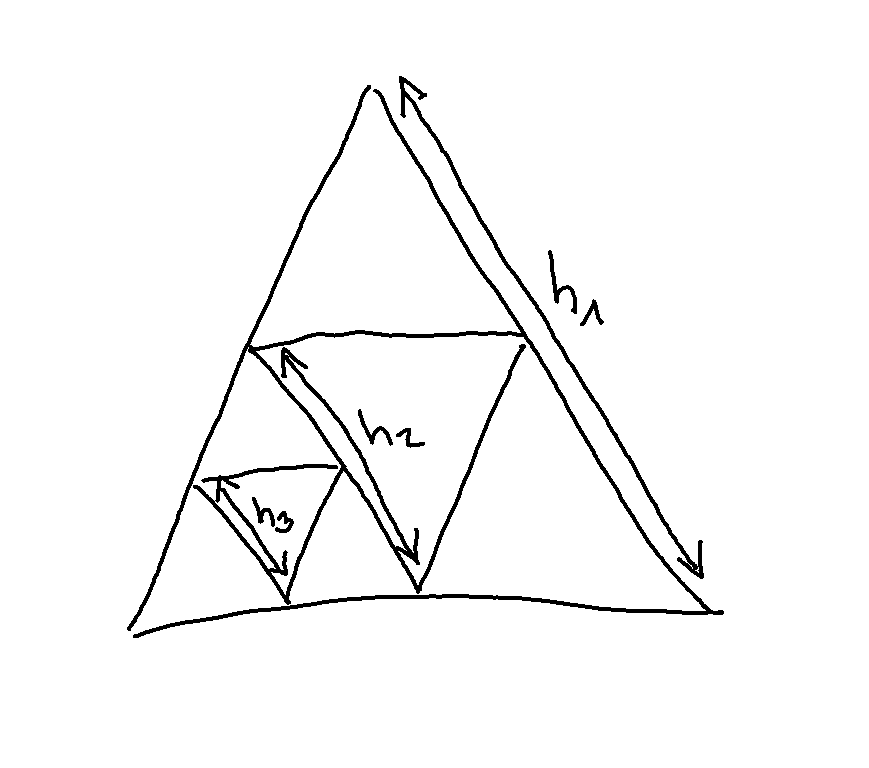
\includegraphics[width=0.75\textwidth]{pics/Sketch3.png}
				\caption{Beispielhafte Verfeinerung der Triangulierung mit einhergehender Konvergenz des Familienparameters}
				\label{AbbFamilienparameterKonvergenz}
			\end{center}
		\end{figure}
	\end{enumerate}
\end{definition}

\begin{theorem}\label{theorem4.16}
	Für eine formreguläre Familie von Finiten-Elementen $(K,V,\Sigma)$, alle affin-äquivalent zu $(\hat{K},\hat{V},\hat{\Sigma})$, ist die Abschätzung
	\begin{align*}
		\big| v-I_K v\big|\leq\tilde{c}\cdot\big(\meas(K)\big)^{\frac{1}{q}-\frac{1}{p}}\cdot h_K^{r+1-m}\cdot|v|_{r+1,p,K}
	\end{align*}
	erfüllt unter den Voraussetzungen von Theorem \ref{theorem4.14}. Außerdem gilt die Abschätzung dann für die Norm anstelle der Semi-Norm:
	\begin{align*}
		\big\Vert v-I_K v\big\Vert\leq\tilde{c}\cdot\big(\meas(K)\big)^{\frac{1}{q}-\frac{1}{p}}\cdot h_K^{r+1-m}\cdot|v|_{r+1,p,K}
	\end{align*}
\end{theorem}

\begin{theorem}\label{theorem4.17}
	Sei $V:=H_0^1(\Omega)$, $V_h\subseteq V$ ein Raum von Finiten Elementen auf $\T_h$ (gehörend zu einer formregulären Familie)  und seien $(K,V,\Sigma)$ affin-äquivalent zu $(\hat{K},\hat{V},\hat{\Sigma})$.\\
	Weiterhin sei $a$ eine koerzive, stetige Bilinearform auf $V$ und $l$ eine stetige Linearform auf $V$.
	Außerdem seien $u\in V$ und $u_h\in V_h$ die 	eindeutigen Lösungen des Variationsproblems auf $V$ bzw. $V_h$.
	Zusätzlich seien $\hat{N}_i\in\hat{\Sigma}$ stetig auf $H^{r+1}(\hat{K})$ und $P_r(\hat{K})\subseteq\hat{V}\subseteq H^1(\hat{K})$\\
	Dann gibt es eine Konstante $c$, unabhängig von $h$ so, dass
	\begin{align*}
		\Vert u-u_h\Vert_{1,2,\Omega}\leq c\cdot h^r\cdot|u|_{r+1,2,\Omega}
	\end{align*}
	unter der Voraussetzung, dass
	\begin{align*}
		u\in H^1_0(\Omega)\cap H^{r+1}(\Omega).
	\end{align*}
\end{theorem}

\begin{proof}
	Céa's Lemma \ref{theorem2.2CeasLemma} liefert
	\begin{align*}
		\Vert u-u_h\Vert_{1,2,\Omega}&\leq c\cdot \inf\limits_{v_h\in V_h}\Vert u-v_h\Vert_{1,2,\Omega}
		\leq c\cdot\Vert u-I_h u\Vert_{1,2,\Omega}
	\end{align*}
	Mit Theorem \ref{theorem4.16} folgt mit $m=1,p=q=2$ dann die Lokalisierungseigenschaft
	\begin{align*}
		\big(I_h v\big)\big|_K&=I_K\big(v|_K\big)\\
		\implies
		\big\Vert u-I_K u\big\Vert_{1,2,K}&\leq c\cdot h_K^r\cdot|u|_{r+1,2,K}\\
		\implies
		\big\Vert u-I_h u\big\Vert^2_{1,2,\Omega}
		&=\sum\limits_{K\in\T_h}\big\Vert u-I_h u\big\Vert^2_{1,2,K}\\
		&=\sum\limits_{K\in\T_h}\big\Vert u-I_K u\big\Vert^2_{1,2,K}\\
		&\leq
		c\cdot\sum\limits_{K\in\T_h}\underbrace{h_K^{2\cdot r}}_{\leq h^{2\cdot r}}\cdot|u|^2_{r+1,2,K}\\
		&\leq c\cdot h^{2\cdot r}\cdot\underbrace{\sum\limits_{K\in\T_h}|u|^2_{r+1,2,K}}_{=|u|^2_{r+1,2,\Omega}}\\
		&=c\cdot h^{2\cdot r}\cdot|u|^2_{r+1,2,\Omega}
	\end{align*}
\end{proof}

\begin{theorem}\label{theorem4.18}
	Zusätzlich zu den Voraussetzungen von Theorem \ref{theorem4.17} nehmen wir hier noch an, dass das Problem
	\begin{align*}
		\text{Finde }\varphi\in V\text{ so, dass }a(v,\varphi)=(g,v)~\forall v\in V.
	\end{align*}
	%provides?
	für alle $g\in L^2(\Omega)$ eine eindeutige Lösung $\varphi_g\in H^2(\Omega)$ hat, die
	\begin{align*}
		\Vert\varphi_g\Vert_{2,2,\Omega}\leq c\cdot\Vert g\Vert_{0,2,\Omega}
	\end{align*}
	erfüllt. Dann existiert eine Konstante $c$, unabhängig von $h$ so, dass
	\begin{align*}
		\Vert u-u_h\Vert_{0,2,\Omega}\leq c\cdot h^{r+1}\cdot|u|_{r+1,2,\Omega}
	\end{align*}
	falls $u\in H^{r+1}(\Omega)$.
\end{theorem}

\begin{proof}
	Nutze Theorem \ref{theorem2.3AubinNitscheDualitaetsargument} mit $H=L^2(\Omega),V=H_0^1(\Omega)$:
	\begin{align*}
		\Vert u-u_h\Vert_{0,2,\Omega}
		&\leq c\cdot\underbrace{\Vert u-u_h\Vert_{1,2,\Omega}}_{\leq c \cdot h^r\cdot|u|_{r+1,2,\Omega}}\cdot\sup\limits_{\begin{subarray}{c}g\in L^2(\Omega)\\\Vert g\Vert_{0,2,\Omega}=1\end{subarray}}\inf\limits_{v_h\in V_h}\Vert\varphi_g-v_h\Vert_{1,2,\Omega}
	\end{align*}
	\begin{align*}
		\implies
		\inf\limits_{v_h\in V_h}\Vert\varphi_g-v_h\Vert_{1,2,\Omega}
		&\leq\big\Vert\varphi_g -I_h\varphi_g\big\Vert_{1,2,\Omega}\\
		&\leq c\cdot h\cdot|\varphi_g|_{2,2,\Omega}\\
		&\leq c\cdot h\cdot\underbrace{\Vert g\Vert_{0,2,\Omega}}_{=1}
	\end{align*}
	\begin{align*}
		\implies
		\sup\limits_{\begin{subarray}{c}g\in L^2(\Omega)\\\Vert g\Vert_{0,2,\Omega}=1\end{subarray}}\inf\limits_{v_h\in V_h}\Vert\varphi_g-v_h\Vert_{1,2,\Omega}
		\leq c\cdot h
	\end{align*}
\end{proof}

Diese Abschätzungen ist eine \textbf{a priori Abschätzung}, d.h. man kann ohne Berechnungen Aussagen machen.

\begin{lemma}[Inverse Abschätzung]\label{lemma4.19InverseAbschaetzung}\enter
Sei $\lbrace V_h\rbrace$ eine Familie von affin-äquivalenten, formregulären Finiten-Elementen.\\
Dann gibt es eine konstante $c$, unabhängig von $h$, so, dass
	\begin{align*}
		|w_h|_{1,2,K}\leq c\cdot h^{-1}_K\cdot\Vert w_h\Vert_{0,2,K}\qquad\forall w\in V_h
	\end{align*}
	Global erhalten wir
	\begin{align*}
		|w_h|_{1,2,\Omega}\leq c\cdot h^{-1}_{\min}\cdot\Vert w_h\Vert_{0,2,\Omega}\qquad\forall w\in V_h
	\end{align*}
	wobei $h_{\min}:=\min\limits_{K\in\T_h} h_K$
\end{lemma}

\begin{proof}
	\begin{align*}
		|w_h|_{1,2,K}
		\overset{\ref{theorem4.9}}&{\leq}
		c\cdot\underbrace{\Vert B_K^{-1}\Vert^1}_{\leq h_K^{-1}}\cdot\big|\det(B_K)\big|^{\frac{1}{2}}\cdot\big|\underbrace{\hat{w}}_{=w_h\circ F_K}\big|_{1,2,\hat{K}}\\
		|\hat{w}_h|_{1,2,\hat{K}}
		&\leq \Vert\hat{w}\Vert_{1,2,\hat{K}}
		\stackrel{(\ast)}{\leq}
		c\cdot\Vert\hat{w}_h\Vert_{0,2,\hat{K}}\\
		\implies
		|w_h|_{1,2,K}
		&\leq c\cdot h_K^{-1}\cdot\big|\det(B_K)\big|^{\frac{1}{2}}\cdot\Vert\hat{w}_h\Vert_{0,2,\hat{K}}\\
		&\leq c\cdot h_K^{-1}\cdot\big|\det(B_K)\big|^{\frac{1}{2}}\cdot\underbrace{\Vert B_K\Vert^0}_{=1}\cdot\big|\det(B_K)\big|^{-\frac{1}{2}}\cdot\Vert w_h\Vert_{0,2,K}\\
		&= c\cdot h_K^{-1}\cdot\Vert w_h\Vert_{0,2,K}
	\end{align*}
	Bei ($\ast$) wird die Normäquivalenz auf endlichen dimensionalen $\hat{V}$ benutzt.
\end{proof}